\chapter{Implementation}
\section{Choices in Technologies}
\label{sec:techchoices}
In this chapter, we outline the technologies we choose, and the reasoning for choosing them.

\subsection{Backend}
\label{subsec:techbackend}
The backend is divided into two parts, the signing service and the verification service.
They are developed independently in different programming languages.

We chose to split the backend into two because signature verification has to be available both online and offline.

Using two different programming languages and sets of libraries,
implementing common formats and protocols independently from specification alone,
allows us to hedge against the risk of some flaws in the libraries: if a library used in the signing service produced flawed output,
it would likely be discovered by the verification service since it uses a different implementation of the same concepts.
The exact same flaw being present in two different libraries implemented in different programming languages is rather small.

On top of that, we can test ourselves how well we've specified the protocols and formats:
if these two services can be used together without problems, the specification was precise enough.
If not, we learn where we must improve it, which is a win-win situation.

\subsubsection{Signing Service}
The signing service is implemented in the Kotlin programming language~\cite{kotlin} using the Ktor framework~\cite{ktor}.
For the signing service we chose Kotlin because it is a modern and concise programming language,
providing null safety, coroutines for asynchronous programming,
support for functional programming with higher-order functions and closures,
and it's genuinely nice to program in.
Kotlin offers seamless Java interoperability, allowing us to make use of the excellent and extensive Java ecosystem.

We haven't picked Kotlin and Ktor at random, we've discussed which language and framework to use for the signing server at length.
The table~\ref{tab:langandfram} lists a short overview which other choices we've discussed but chosen not to pursue.

\begin{figure}
    \begin{center}
        \begin{tabular}{p{1.5cm}|p{2cm}|p{11cm}}
            \textbf{Language} & \textbf{Framework} & \textbf{Reason for non-consideration} \\
            \hline
            Java & Spring MVC & Steep learning curve, vast amount of functionality to learn, too large for our needs, little previous knowledge on our part \\
            \hline
            Java & Vaadin & Generated frontend is slow to use because of network latency, too much uncertainty with regards to \gls{WASM} integration: Is it possible? How? How long will it take us, how much will we have to implement ourselves? \\
            \hline
            C\# & .NET Core & Zero previous knowledge on our part both for the language and the framework, aversion to Microsoft because of their attempts to undermine open-source software~\cite{mseee} \\
            \hline
            Scala & Play & Little previous knowledge of the language, uncertainty of the time required to learn it properly, but otherwise an interesting contender \\
            \hline
            Python & Django & Huge framework to learn, no type safety, slow runtime performance \\
        \end{tabular}
        \captionof{table}{Programming languages and frameworks considered for use in the signing service implementation\label{tab:langandfram}}
    \end{center}
\end{figure}


\subsubsection{Verifier}
The verification service is implemented in the Go programming language~\cite{golang}.
For the verifier we chose Go,
because it allows us to generate statically linked binaries for all major platforms,
without worrying about dependencies.
Further the Go standard library already includes a lot of cryptographic functionality,
requiring fewer third party dependencies.
Go's built-in concurrency primitives (goroutines and channels) make it easy implement the verification of the many parts of the signatures asynchronously.
With only having a single \gls{API} endpoint for verifying the signature it isn't necessary to use a complicated web framework as the \texttt{http} package of the Go standard library provide all needed functions.

As with the signing service implementation, we evaluated alternatives, which are summarised in table~\ref{tab:goalts}.

\begin{figure}
    \begin{center}
        \begin{tabular}{p{1.5cm}|p{2cm}|p{11cm}}
            \textbf{Language} & \textbf{Framework} & \textbf{Reason for non-consideration} \\
            \hline
            Java & JavaFX & Requires the user to either have Java installed or will be bundled with the program, which makes it quite large.  \\
            \hline
            Anything & Electron & Electron is ludicrously resource-hungry, having the Chromium engine underneath. It also requires more frontend (javascript) code than any of us is comfortable with. \\
        \end{tabular}
        \captionof{table}{Programming languages and frameworks considered for use in the verification service implementation\label{tab:goalts}}
    \end{center}
\end{figure}


\subsection{Frontend}
\label{subsec:techfrontend}

Given that the frontend must support the three desktop operating systems Microsoft Windows,
GNU/Linux as well as Apple MacOS,
the technological choices available to us are limited.
On the desktop, we could use the \gls{JVM} platform and the JavaFX \gls{GUI} library, whereas on the phones
we could use Flutter~\cite{flutterframework}.
However, developing three applications on five platforms using two new-to-us frameworks and programming languages
would take a lot more time and resources than what is available to us in the scope of this thesis.

In order to reduce complexity and enable code reuse, we decide to implement the frontend as a web application.
Web frontents are capable of running in any modern web browser regardless of platform, be it mobile or desktop.
We're not happy about this, as we would much rather use mature, strongly-typed and well-designed languages and frameworks,
but we're forced to make this compromise in order to meet our objectives in the time available.
In order to reduce the pain, we will use TypeScript, which is a typed superset of JavaScript~\cite{loltypes}.
We discussed implementing a \gls{SPA} using Angular~\cite{angular},
but for our use case it's overkill as there isn't too much client-side logic.
In the interest of a small, fast-loading site we chose to stick with plain \gls{HTML} and \gls{CSS}
and only adding as much JavaScript as necessary.

\subsection{Client-Side File Hashing in the Web Browser}
\label{subsec:browserhashing}
However, the decision to implement the frontend as a web application presents us with a challenge:
hashing the files to be signed client-side in the web browser itself.
If we had implemented "proper" client applications this would've been easy, but in a web browser and using its
JavaScript language not so much: it simply wasn't designed with performance in mind.

The easiest solution would be to upload the files to be signed to the server and hash them there,
but this would be a clear violation of the least-information principle (the server doesn't need the file, only the hash)
and a breach of user privacy.
Nevermind the fact that signing large files could take a very long time over slow network connections,
and turn out to be quite expensive for mobile users billed for data by volume.

Another solution would be to ask the user to enter the file hashes instead of selecting files,
but this would be very user-unfriendly and most likely too much to ask from many users.

It is clear we must find a way to hash files in the web browser itself.
In order to achieve this we have found the following options:

\begin{enumerate}
    \item Using the browser-implemented \texttt{SubtleCrypto}~\cite{subtlecrypto} \gls{API}
    \item Using the \texttt{CryptoJS}~\cite{cryptojs} JavaScript implementation
    \item Using a \gls{WASM}-based implementation
\end{enumerate}

Each of these options comes with a number of advantages and disadvantages, as discussed in more detail in the following sections.

\subsubsection{Using SubtleCrypto}
\label{subsec:subtlecrypto}
The \texttt{SubtleCrypto} class offers the \texttt{digest(algorithm, data)} method~\cite{subtlecrypto}, which can be used to
calculate \gls{SHA-256} checksums.
The advantage of using this implementation is that it is available in all modern browsers\footnote{Where modern browsers means Mozilla Firefox, Google Chrome/Chromium, and Microsoft Edge, not older than the respective versions available in 2018},
and since it's executed with native code, being able to take advantage of \gls{AVX2} instructions, instead of JavaScript it should be quite fast.
There's a major drawback though: hashing a large amount of data progressively is not supported, the data has to be
passed to the function en bloc, as seen in listing~\ref{lst:subtlecrypto}.

\lstinputlisting[caption={Using SubtleCrypto for calculating SHA-256 checksums}, captionpos=b, language=JavaScript, label={lst:subtlecrypto}]{listings/subtlecrypto.js}

Our testing showed that selecting files larger than 200MB crashes Firefox tabs when trying to read their contents
into memory before we could pass it to the \texttt{digest} function.
If we assume the users will only ever select small files this should not pose a problem, but unfortunately it's not safe to assume this.
Furthermore, this limit is probably lower still on mobile devices such as smartphones (although we didn't test this).

\subsubsection{Using CryptoJS}
\label{subsec:cryptojs}
\texttt{CryptoJS} does not have the limitation of \texttt{SubtleCrypto} and supports progressive hashing\footnote{
By progressive hashing we mean the ability to pass to the hash function the data piece by piece in order to avoid holding all of it in memory at once.},
as seen in listing~\ref{lst:cryptojsprogressive}.

\lstinputlisting[caption={Progressive SHA-256 hashing using CryptoJS},captionpos=b,language=JavaScript,label={lst:cryptojsprogressive}]{listings/cryptojs.js}

The advantage of using \texttt{CryptoJS} over \texttt{SubtleCrypto} is, as mentioned, the ability to hash piece-wise.

The disadvantage is that we need to load a third-party JavaScript library, using built-in functionality would be preferable.

And since JavaScript is an interpreted language, using it to calculate the checksums results in performance figures everyone but web developers would laugh at.
This is a problem especially on mobile devices limited in compute and memory resources as well as battery capacity.
Since we want to support mobile devices properly, and don't want to limit users to small files, we must do better.

\subsubsection{Using a WASM-based implementation}
\label{subsec:wasmhashing}
\gls{WASM} provides a low-level virtual machine in the web browser itself,
running machine-independent binary code, comparable to the \gls{JVM} or the \gls{CLR},
albeit much simpler and much less sophisticated.
By using this virtual machine we should be able to run code at near-native speed written in a statically-typed, compiled language such as Rust, C/C++ or Go.
Thus we expect significant performance gains over a JavaScript-based implementation.
While developing the \gls{WASM}-based hashing programmes, we encountered some interesting challenges, as described in the following paragraphs.

\paragraph{CORS Policy} While JavaScript can be executed simply by pointing the browser at a local \gls{HTML} file, the same doesn't work for \gls{WASM}.
The browser's security policy forbids it due to its \gls{CORS} rule~\cite{cors}.
We solved this by starting the \gls{HTTP} server built in to Go's standard library and having the browser load the \gls{WASM} binary through \gls{HTTP}.
The code is in appendix~\ref{chap:appendix_golangwebserver}.
For the Rust-based implementation we used the built-in web server of webpack~\cite{webpack}.

\paragraph{JavaScript/WASM Compatibility} The Golang project conveniently provides a file containing the necessary boilerplate code to load, start and interact with \gls{WASM} programmes called \texttt{wasm\_exec.js}.
But there's a catch: for each version of Go, the version of the accompanying \texttt{wasm\_exec.js} file used must match precisely.
If it doesn't, the code will crash with a segmentation fault.
It took us quite some time to figure out why the code we'd written only a few days prior would segfault now with no changes made to it.

\paragraph{Passing data} Functions written in Go intended to be used from the JavaScript side of things need to have a very specific signature.
As can be seen in listing~\ref{lst:funcsignaturewasm}, there is no typing: all arguments passed to the function are of type \texttt{js.Value} and the return value must be of type \texttt{interface\{\}}\footnote{\texttt{interface\{\}} is Go's equivalent of Java's \texttt{Object}, it could be anything.}.
This posed us with the challenge of detecting the types and casting the data passed accordingly.

\lstinputlisting[caption={Golang WASM function signature}, captionpos=b, language=Go, label={lst:funcsignaturewasm}]{listings/wasmfunc.go}

We've worked on this for hours, producing ugly reflection-based hacks, until we decided to just agree on the types of the arguments and return values beforehand despite the open function signature.
Now all that's needed is a little boilerplate to convert a JavaScript \texttt{Uint8Array} to a Golang \texttt{[]byte}, as seen in listing~\ref{lst:jscastingtogo}.

\lstinputlisting[caption={Uint8Array to {[]}byte}, captionpos=b, language=Go, label={lst:jscastingtogo}, captionpos=b]{listings/jscasting.go}

\paragraph{Goroutines} Go features its own concurrency primitive called Goroutines.
From a programmers' perspective, they can be used like threads, but they carry much less overhead.
Communication between goroutines is achieved by using so-called channels, which on a high level are comparable to queues.
Unfortunately, the \gls{WASM} specification wasn't drafted with this kind of concurrency in mind.
Go is forced to unwind and restore the call stack when switching between goroutines, which is very expensive~\cite{lolnogoroutines}.
We rewrote the Go programme to work without them, and we've seen a small but significant performance improvement.

\paragraph{Rust based WASM}
As the Go implementation also includes the Go runtime,
which makes the wasm file much larger,
and starts a programme that will run continuously in the background it isn't the optimal choice for creating a WebAssembly implementation.
As neither of us knows any other of the other languages that compile to WebAssembly well, we excluded them at first.
However with the drawbacks of the Go based implementation we decided to try to implement a Rust-based version as well,
in order to see how they compare both in performance and ease of development.


\subsubsection{Performance Comparison}
\label{subsec:perfcomphashing}
No one likes waiting for slow software to do its work, and neither do we.
This is why we decided to compare the performance of the aforementioned options in a simple test:
we measure the time it takes for the browser to calculate the checksum of 1GB of random data using the aforementioned methods.
The code used for each example is in appendix~\ref{ch:appendix-in-browser-hashing-code}.
The tests were run on Debian 10 using Firefox 69 on an Intel i7-8550U.
The results can be seen in figure~\ref{fig:hashingperformance}.

As expected, the in-browser \texttt{SubtleCrypto}-implementation is the fastest, followed by the Rust-based implementation.
JavaScript is so ridiculously slow it's not even trying to compete.
In order to provide a reference to compare the hashing speeds to we include the performance of the \texttt{openssl} command-line programme.

\begin{figure}
    \begin{center}
        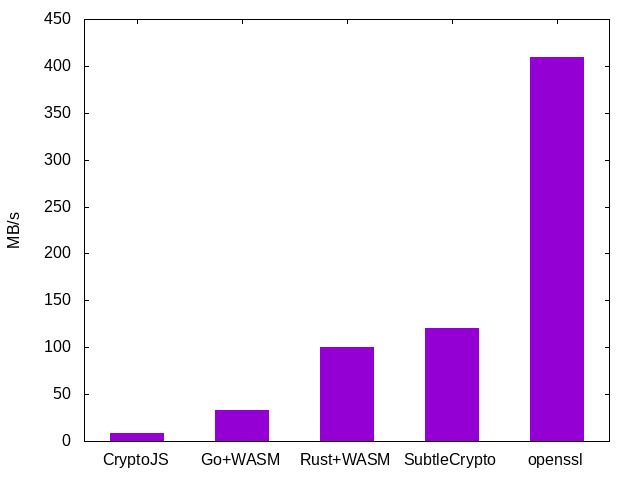
\includegraphics[width=0.7\linewidth]{images/hashingperformance.png}
        \caption{Hashing speed in MB/s (higher is better)}
        \label{fig:hashingperformance}
    \end{center}
\end{figure}


\subsection{Deciding On The In-Browser Hashing Implementation}
\label{subsec:deciding-on-the-in-browser-hashing-implementation}
It is clear from figure~\ref{fig:hashingperformance} that \texttt{SubtleCrypto} is the fastest of the options we tried.
Unfortunately, since it doesn't support piece-wise hashing we're forced to pick the next-fastest option,
the Rust-based implementation running in the \gls{WASM} \gls{VM}.
Using Rust provides us with another significant advantage:
the toolchain is highly developed.
Upon compilation, the toolchain auto-generates TypeScript declaration files containing the function signatures
the \gls{WASM} module exposes to the JavaScript world.
This is very nice, since it allows for compile-time type checking and for smarter code completion in the \gls{IDE},
as shown in figure~\ref{fig:dtside}.

\begin{figure}
    \begin{center}
        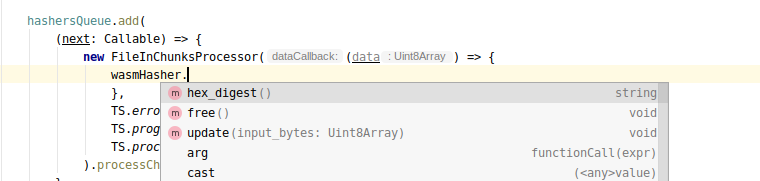
\includegraphics[width=0.7\linewidth]{images/dtside.png}
        \caption{Code Completion in Intellij}
        \label{fig:dtside}
    \end{center}
\end{figure}


\subsection{Software Libraries}\label{subsec:software-libraries}
Table~\ref{table:libraries} summarises the software libraries used in the implementation of the signing service.
All libraries we use are of high maturity, widely used, well tested and above all,
free and open source software.
That is, they are licenced with \gls{FSF} approved open source licences.

\begin{figure}
    \begin{center}
        \begin{tabular}{p{3cm}|p{12cm}}
            \textbf{Name} & \textbf{Description} \\ \hline
            logback &
            An implementation of the \gls{SLF4J} \gls{API}.
            It's a replacement for log4j, but brings a large number of improvements.
            Also, it's Swiss, which we found nice.
            We use it as the \gls{SLF4J} implementation.
            \\ \hline
            Apache HttpClient &
            Ktor's built-in \gls{HTTP} client isn't usable on its own,
            it requires a backing engine.
            We've selected the Apache HttpClient for this.
            Other alternatives were \gls{CIO}, Jetty, and OkHttp.
            It's probably the most configurable and complete \gls{HTTP} client available at the time of writing. It supports both \gls{HTTP}/1.1 and \gls{HTTP}/2,
            and is the only one available that supports following redirects and allows for configuration of timeouts and proxies.
            \\ \hline
            kotlinx.serialization &
            Kotlin Serialization is comparable to Jackson in that it provides serialisation of \gls{JSON},
            but unlike Jackson,
            it works without reflection.
            Instead it's implemented as a compiler plugin and a runtime library.
            The compiler plugin automatically generates the visitor code for the data classes,
            while the runtime library uses the generated code for serialisation without reflection.
            This massively improves runtime performance.
            \\ \hline
            JUnit &
            JUnit is probably the most widely used unit testing framework in the Java ecosystem.
            We use it to write our unit tests with it,
            as it provides convenient integration into Ktor.
            \\ \hline
            Bouncy Castle &
            Bouncy Castle is an extensive cryptography library for Java (and C\#).
            We use it extensively in the signing service:
            to build \gls{CMS} messages,
            to generate \gls{RSA} keys,
            to work with X.509,
            to create \gls{OCSP} and \gls{TSP} requests and read the responses,
            and more.
            Without this library we couldn't have achieved what we did.
            Unfortunately, the documentation isn't very good (sometimes non-existent),
            and we've spent a lot of time figuring out how to use it correctly.
            \\ \hline
            auth0 jwt/jwks &
            Java implementations of the \gls{JWKS} and \gls{JWT} standards,
            used for \gls{OIDC} integration and id\_token verification.
            We haven't looked for alternatives because this library works well,
            has on-point documentation, and is MIT-licenced.
            \\ \hline
            jsoup &
            Jsoup is a library for working with \gls{HTML}.
            It provides a well-designed \gls{API} for extracting data from the \gls{DOM},
            using jquery-like methods.
            We use it to submit the login form on the Keycloack \gls{IDP} in the unit tests.
            We can't POST the form directly because there is a hidden \gls{CSRF} token field in the form,
            whose value we have to extract.
            This is what jsoup is good in.
            \\ \hline
            protobuf &
            This is the reference implementation of protocol buffers.
            We use it to build the signature file.
            \\ \hline
            Koin &
            Insert-Koin is a pragmatic, light-weight dependency injection framework for Kotlin.
            What distinguishes it from other \gls{DI} frameworks,
            and in our opinion makes it better,
            is that it uses purely functional resolution.
            There is no reflection, no proxies, and not even code generation.
            \\
        \end{tabular}
        \captionof{table}{Software libraries used in the development of the signing service\label{table:libraries}}
    \end{center}
\end{figure}

\subsection{Software Libraries - Verification Service}\label{subsec:software-libraries-verifier}
Table~\ref{table:libraries} summarises the software libraries used in the implementation of the verification service.
As with the libraries for the signing service,
they are all of high quality and free and open source software.
In some cases, we needed to fork a library and extend functionality for which we created pull requests in the respective project repositories.
For more information about our contributions to open source software during this thesis see TODO document PRs and link here.

\begin{figure}
    \begin{center}
        \begin{tabular}{p{4.2cm}|p{12cm}}
            \textbf{Name} & \textbf{Description} \\ \hline
            github.com/sirupsen/logrus & A structured logger, that is API compatible with the Go standard library logger. Used so we don't have to do the log formatting all by ourself. \\
            \hline
            go.mozilla.org/pkcs7 & Library for parsing and verifying \gls{PKCS7}/\gls{CMS} and RFC3161\cite{rfc3161} timestamps. As the library only supported \gls{CRL}s for checking the revocation data, we added support for \gls{OCSP}. \\
            \hline
            gopkg.in/square/go-jose.v2 & Implementation of the \gls{JOSE} set of standard like \gls{JWT} and \gls{JWK}. Used for extracting the X.509 certificates from the \gls{JWK}s in the signature data and for verifying the ID token signature. \\
            \hline
			github.com/coreos/go-oidc & Used for verifying and parsing the \gls{OIDC} ID tokens. \\
            \hline
            github.com/golang/protobuf & Reference implementation of protocol buffers, which are used in our signature format. \\
            \hline
            golang.org/x/crypto & Extended part of the Go standard library. Mainly used for parsing and verifying \gls{OCSP} responses. \\
            \hline
            github.com/shurcooL/vfsgen & Generates go "code" from static files and makes them accessible via a virtual filesystem. This is used to work around Go's limitation of not being able to embed files in the compiled binary.
        \end{tabular}
        \captionof{table}{Software libraries used in the development of the verification service\label{table:libraries-verifier}}
    \end{center}
\end{figure}


\subsection{Dependency Management}\label{subsec:dependency-management}
For the signing service's dependency management,
we use Apache Maven~\cite{mvn}.
It allows us to specify project metadata,
build configuration,
and of course build- and runtime dependencies in a central location.
Most Java developers are familiar with Maven and should be able to feel right at home.
We chose Maven over alternatives such as Gradle and Ant because it is the most widely used dependency and build management system available in the Java world.

For the verifier,
we use Go's built-in module system.
A Go module is a set of Go packages in a file tree with a \texttt{go.mod} file at the root of the tree.
This file defines the dependency requirements,
which are pulled by the Go build system before compilation.
A go package has a import path, which is actually an url path, where the package source is hosted.
At this path the go tool expects to be a source repository (git, svn, mercurial) with the tagging system of the \gls{VCS} used for determening the version (if any).

For the frontend we have to combine two dependency management tools.
\paragraph{npm} The node package manager is used to install the TypeScript compiler \texttt{tsc},
which type-checks, then translates the TypeScript source code into JavaScript.
We also use \texttt{webpack},
a tool which allows us to combine all of the compiled JavaScript files into a single bundle file.
The code in that bundle file is minified,
a process in which the code is transformed in such a way as to be as small as possible.
This reduces the amount of data that has to be transmitted over the network.

\paragraph{Cargo} Cargo is the package manager for the Rust programming language.
It downloads dependencies, compiles packages,
and builds binaries ready for distribution.
We use Cargo to build the \gls{WASM}-based in-browser hashing binary,
which in turn is used by the frontend of the signing server as well as the verifier.

\subsection{Software Packaging}\label{subsec:software-packaging}
For the signing service,
we use the \texttt{shade} plugin for Maven.
This plugin allows us to package our artifact into a \gls{JAR},
including all runtime dependencies and resources.

For the signing server,
the resource files that have to be included into the production-ready \gls{JAR}
are the frontend files (\gls{HTML}, \gls{CSS}, \gls{JS} and \gls{WASM}),
as well as the Ktor configuration file.
This allows for simple deployment:
all that's needed on the target server is a \gls{JRE},
and the rest is contained in the \gls{JAR}.
The admin doesn't even have to set up Tomcat,
and running the server is as easy as executing \texttt{java -jar signingserver-shaded.jar}.

Go uses static linking by default,
it even includes its own \gls{VM} into the binaries it builds.
This has the advantage of vastly simplified deployment:
all anyone needs to do is to copy the binary and run it.
The downside is that the binary is somewhat larger.

However, Go's build system doesn't support including additional files in that single binary.
As a workaround, we've used the \texttt{vfsgen} library.
For a given set of files and directories represented as the \texttt{http.FileSystem} interface,
it generates Go code that statically implements that interface,
which in turn is used just like any other Go package.
The end result is one single executable file which contains everything it needs,
even its own runtime, unlike the fat \gls{JAR} which doesn't work without a \gls{JRE}.

\subsection{Custom Docker Image for Rust+Webpack Build}\label{subsec:custom-docker-image-for-rust+webpack-build}
Gitlab \gls{CI} uses docker images as the build environment in which to compile and package artifacts.
For all but one of our components we were lucky enough to find pre-built images providing what we needed (for example, a Maven 3 environment).
Unfortunately it seems with Rust + Webpack we're a bit on the forefront of things,
and no one's published a usable docker image for that build configuration to Dockerhub yet.

This is why we built our own image on top of a base Ubuntu+Rust image by adding the following:
\begin{enumerate}
    \item Installing \texttt{curl}
    \item Installing \texttt{wasm-pack}.
    This tool implements the workflow necessary for building Rust into \gls{WASM},
    generating the \gls{JS} and TypeScript binding code,
    and generates npm packages ready to be included into our project.
    \item Installing \texttt{cargo-generate}, a scaffolding tool which generates the boilerplate necessary for Cargo to work.
    \item Installing \texttt{npm}, the node package manager.
\end{enumerate}

We published this image onto Dockerhub as \texttt{izolight/rust-webpack},
hoping that others might find it useful.

\subsection{Combined Build Process}\label{subsec:combined-build-process}
Since we use so many languages, tools and frameworks,
the build process gets a bit complicated.
For this reason we document it here.

\begin{enumerate}
    \item \texttt{npm} downloads and installs the \texttt{webpack} and TypeScript toolchains
    \item \texttt{wasm-pack} calls \texttt{Cargo},
    which downloads and installs the Rust dependencies,
    and compiles the \gls{WASM} binaries
    \item \texttt{wasm-pack} generates glue code allowing for \gls{WASM} to \gls{JS} bindings
    \item \texttt{webpack} starts \texttt{tsc}, which typechecks,
    then translates the TypeScript source code into JavaScript.
    Then, it combines the generated \gls{JS} from \texttt{tsc} as well as \texttt{wasm-pack} into a minified bundle file,
    and packages it together with the \texttt{HTML} and \texttt{CSS} files.
    \item The verifier uses \texttt{go generate} to compile the frontend files it requires into a Go module,
    which were built in steps 1-4
    \item The signing server copies its frontend files built in steps 1-4 into its resources directory,
    then calls Maven to build its fat \gls{JAR}.
    \item The verifier calls \texttt{go build} three times,
    once respectively for GNU/Linux, Mac OSX and Windows,
    resulting in the binaries for each platform.
\end{enumerate}


Figure~\ref{fig:pipelines} illustrates the combined build process as implemented in Gitlab \gls{CI}.


\begin{figure}
    \begin{center}
        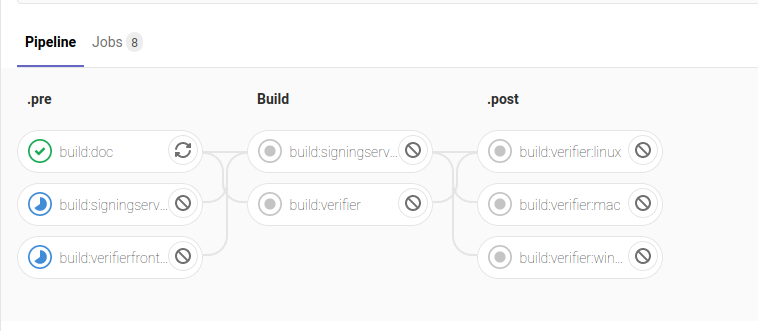
\includegraphics[width=0.7\linewidth]{images/pipelines.png}
        \caption{Gitlab CI pipelines combining different build tools and the artifacts they produce}
        \label{fig:pipelines}
    \end{center}
\end{figure}

\section{Implementation Components}\label{sec:implementation-components}
\subsection{Design Principles}\label{subsec:design-principles}
We've split the implementation of the Signing Service and the Verifier into small,
replaceable modules with clearly defined interfaces.
We've done this to achieve clear separation of concern and loose coupling,
in the spirit of the Law of Demeter~\cite{demeter}.

\paragraph{The Law of Demeter} is a well-known heuristic that states that any module should not know about the
internals of the objects it manipulates.
It is a special case of Loose Coupling.
Objects should hide their data, and expose operations.
This makes it easy to add new types of objects without requiring changing existing behaviours.
It also makes it hard to add new behaviours to existing objects.
Data structures should expose data and have no significant behaviour.

\paragraph{Loose Coupling} refers to the degree of knowledge that one component has of another.
Structuring programs to consist of components that know little of one another
results in easy-to-understand, easy-to-test code.
Developers new to the project can start with work on a small module and don't need to understand the whole system.
Refactoring (or replacing) the implementation of a component becomes easy,
as there are clear boundaries,
and changing the implementation of one component does not affect the others as long as
the boundary contract remains satisfied.


\paragraph{Inversion of Control} enables us to remove the few interdependencies remaining in the modules:
knowing about each other.
A component should not care about where, how and why another component is implemented,
it should only care about being provided the behaviour it requires.
Inversion of Control through Dependency Injection allows each component to declare
its dependencies through interfaces,
and having it supplied the implementation of that interface from the system it is part of,
without knowing anything whatsoever about that implementation.

Applying these methodologies doesn't guarantee clean code, nothing does.
However in our experience, modularisation, decoupling, and separation of concerns is the best single principle
to apply to software development to achieve some level of code quality.

\subsection{Components of the Signing Service}\label{subsec:modules-of-the-signing-service}
There are two groups of components in the signing service:
\begin{itemize}
    \item The views: They implement the \gls{REST} interface to the outside world.
    \item The services: Replaceable components providing functionality needed by the views in order to
    be able to meet their purpose.
\end{itemize}

For a \gls{UML} component diagram showing a simplified overview of the components, see figure~\ref{fig:signingservicecomponents}.

\begin{figure}
    \begin{center}
        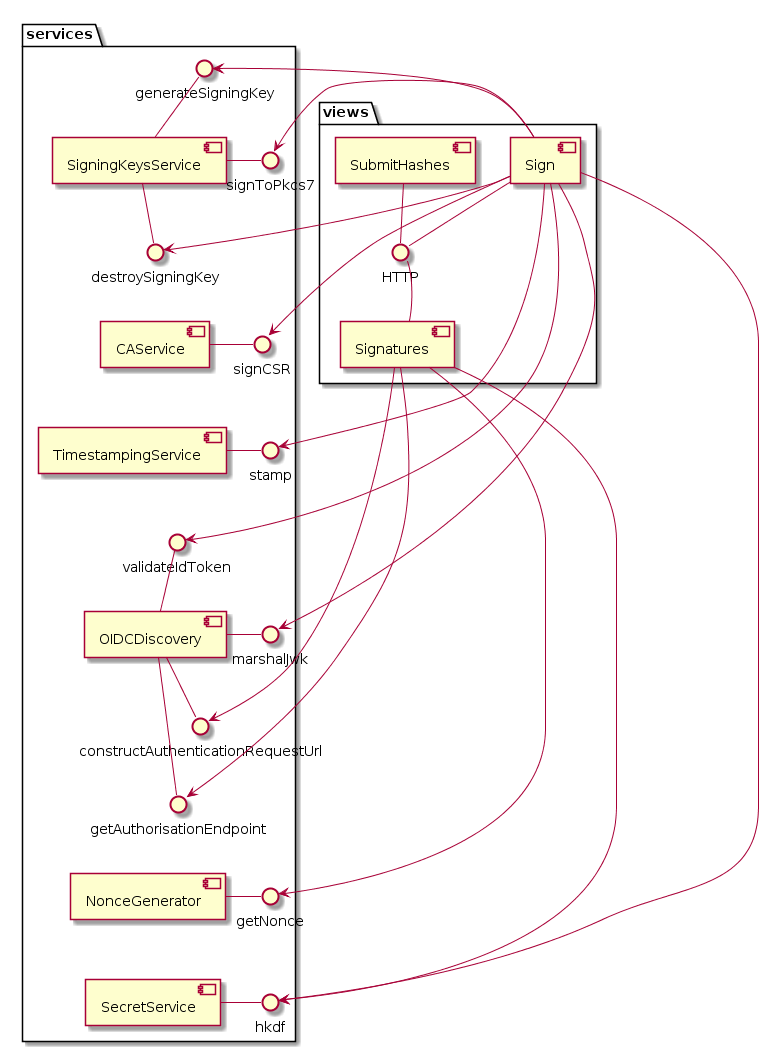
\includegraphics[width=0.7\linewidth]{images/signing_service_components.png}
        \caption{Signing Service Components}
        \label{fig:signingservicecomponents}
    \end{center}
\end{figure}


\subsection{Components of the Verifier}\label{subsec:modules-of-the-verifier}
The verifier has an embedded webserver with a single \gls{API} endpoint.
The webserver handles the \gls{HTTP} side of things.
It interfaces with the verifier modules, which are split by responsability (e.g. \texttt{id\_token} verification).
For a \gls{UML} component diagram showing a simplified overview of the components, see figure~\ref{fig:verifiercomponents}.

\begin{figure}
    \begin{center}
        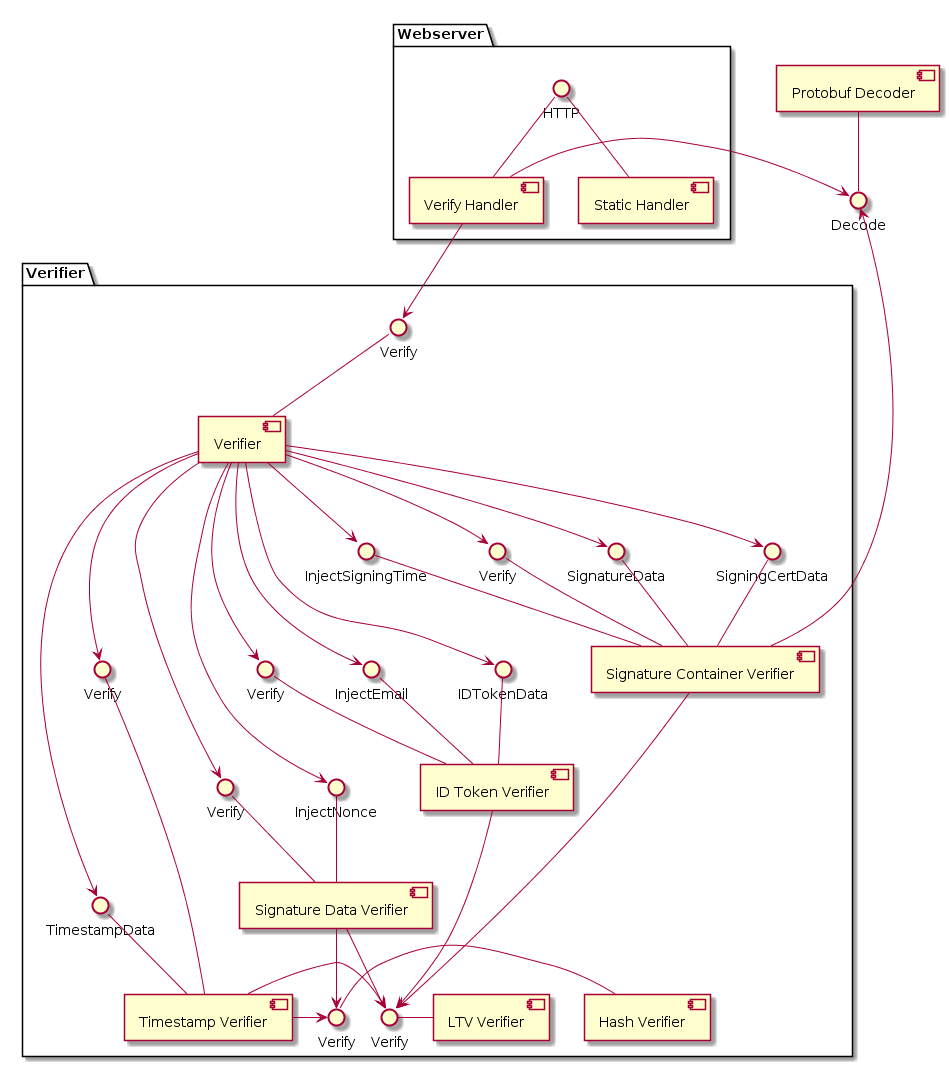
\includegraphics[width=0.7\linewidth]{images/verifier_components.png}
        \caption{Verifier Components}
        \label{fig:verifiercomponents}
    \end{center}
\end{figure}



\section{Finding services fitting our requirements}\label{sec:finding-services-fitting-our-requirements}

For our remote signing service to work,
we need an \gls{IDP} satisfying the requirements documented in section~\ref{sec:requirements-for-idps},
a \gls{TSA} willing to timestamp our signatures,
and a \gls{CA} with an \gls{OCSP} responder that will sign our certificates.

\subsection{Finding a TSA}\label{subsec:finding-a-tsa}
Searching for publicly available \gls{TSA}s, we've found a list as part of the software-library~\texttt{python3-rfc3161ng}~\cite{pythonrfc3161}:
\begin{itemize}
    \item \url{http://freetsa.org/tsr}
    \item \url{http://time.certum.pl}
    \item \url{http://timestamp.comodoca.com/rfc3161}
    \item \url{http://timestamp.geotrust.com/tsa}
    \item \url{http://timestamp.globalsign.com/scripts/timstamp.dll}
\end{itemize}

However we went with the SwissSign \gls{TSA}, as it seemed the least untrustworthy to us.

It worked as expected the first time we tried requesting a timestamp from it.
We used the \texttt{openssl ts} command line program.
Furthermore, to our knowledge, it is available free of charge,
and during our development and testing they didn't restrict us as to the number of timestamps we requested,
which was good enough for our \gls{POC}.

It can be found at \url{http://tsa.swisssign.net}.

We construct the timestamping requests using the \texttt{TimeStampRequestGenerator} class from BouncyCastle~\cite{timestamprequestgenerator},
which works well.

\subsection{Finding an IDP}\label{sec:finding-an-idp}
Finding an \gls{IDP} prividing such strong guarantees as required for Swiss citizens was not easy,
we were able to find only one: SwissID.
We searched online for documentation from them on how we could integrate their \gls{IDP} into our project,
but we could find none.
So we sent them an e-mail and asked, and got a phone call from one of their key account managers,
who seemed to understand little of our actual request but wanted to send us a whitepaper.
That turned out to be marketing material with very little technical information and quite useless to us.
Fearing the sudden appearance of a very large bill we stopped communicating with them.

For the purposes of our \gls{POC} and in the interest of having a working demo soon,
we don't really need an \gls{IDP} with actual guarantees, we just need any working \gls{OIDC} \gls{IDP}.

That led us to search for publicly available \gls{IDP}s that we could use free of charge,
with self-onboarding and readily-available online documentation.

We found the following:
\begin{itemize}
    \item Github: Doesn't support \gls{OIDC}, only OAuth
    \item Yahoo, Paypal, Salesforce, Phantauth, Okta, Google: Don't use X.509
    \item Microsoft: Uses X.509, but the intermediate certificate is self-signed. Why they're doing that is unclear to us, it seems futile.
\end{itemize}

So, in the end, unfortunately we didn't find a single free-of-charge \gls{IDP} that we could use.
Thus we were forced to set up our own.
For this purpose we selected Keycloak, a powerful \gls{IDM}, developed by Red Hat~\cite{keycloak}.
Keycloak is highly configurable and allowed us to run exactly the \gls{IDP} we needed.
For the duration of our thesis, it can be found at \url{https://keycloak.thesis.izolight.xyz/auth/realms/master/.well-known/openid-configuration}.

\subsubsection{Infrastructure setup for the IDP}
It would've been easy to run Keycloak on our local machines, and for the demo this would've been enough,
but we wanted to do it properly, with an internet-accessible \gls{IDP}.
To achieve this, we needed an internet-accessible server, a certificate for \gls{HTTPS},
and \gls{DNS} entries.

For the server, we chose Scaleway's development server simply because it costs as little as 3 EUR per month~\cite{scaleway}.
For certificates, we used the excellent Let's Encrypt \gls{CA}~\cite{letsencrypt}, which is a trusted \gls{CA} issuing domain validation certificates free of charge.

\begin{figure}
    \begin{center}
        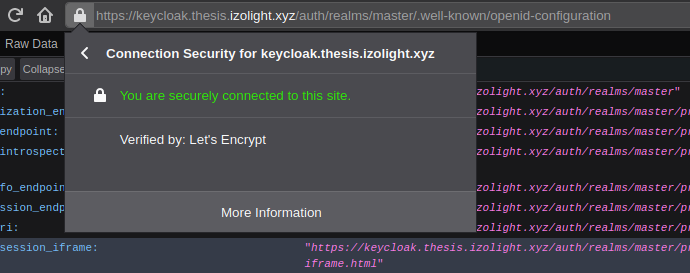
\includegraphics[width=0.7\linewidth]{images/firefox.png}
        \caption{Firefox trusting the certificate issued by the free and open CA Let's Encrypt}
        \label{fig:letsencrypt}
    \end{center}
\end{figure}

This only left us with \gls{DNS}.
Fortunately Gabor Tanz already runs his own \gls{DNS} server for other purposes (and also owns a domain),
so we simply added the appropriate subdomain entries and we were ready to proceed.


\subsection{Finding a CA}\label{subsec:finding-a-ca}
Unfortunately, Let's Encrypt doesn't issue signing certificates~\cite{letsencryptfaq}, only domain validation certificates.
We didn't spend much time searching for other \gls{CA}s since we expected to find none that issues
signing certificates in an automated way and free of charge.
Consequently we proceeded to set up our own \gls{CA}, as we did with the \gls{IDP}.
This meant more of an up-front investment of time,
but better predictability of efforts since everything would be under our control,
if we'd run into any issues.

To set up our own \gls{CA}, we selected Cloudflare's \texttt{cfssl} \gls{PKI} toolkit~\cite{cfssl}.
There was no evaluation of which software to use,
since at this point we were behind schedule
(because we spent more time on the concept part than we planned in order to get multi-signatures right).
We weren't keen on spending much more time on evaluating the \gls{CA} toolkit to use because it'd be relevant for the \gls{POC} only anyway,
and it didn't matter too much as long as it fulfilled its purpose.
On top of that we already had some knowledge of \texttt{cfssl}.

On the same server we'd already spun up to host our \texttt{Keycloak} \gls{IDP},
we installed \texttt{cfssl}.

\subsubsection{Separation of services using Docker containers}


In order to have some separation between the different pieces of software we decided to use Docker.

Table~\ref{tbl:docker} contains a complete list of Docker containers running on our server.
For a graphical representation, please see figure~\ref{fig:infrastructurebigpicture}.

%\paragraph{\texttt{traefik}} is an open-source edge router implementation.
\paragraph{traefik} is an open-source edge router implementation.
It receives outside requests on behalf of the actual system,
finds out which service is responsible to handle them,
and then passes them on.
It is able to automatically discover configuration and provide its routing accordingly,
and it can act as a \gls{HTTPS} termination point.
This helps lessen the load on backend components.
In our case, it takes \gls{HTTPS} requests, figures out which container is responsible for handling it,
and passes it on as \gls{HTTP} (thus terminating \gls{TLS}).


\paragraph{Keycloak} is the \gls{IDP}, and \texttt{keycloak-db} contains its PostgreSQL database.
\paragraph{cfssl-root} and \texttt{cfssl-intermediate} contain the respective root and intermediate certificates,
and serve certificate signing requests.
The containers with the \texttt{-db} suffixes run their PostgreSQL databases, same as for keycloak.
The intermediate \gls{CA} exposes a \gls{REST} \gls{API} used by the signing server.
\paragraph{cfssl-root-ocsp} and \texttt{cfssl-intermediate-ocsp} contain the \gls{OCSP} responders,
which handle \gls{OCSP} requests for certificates issued by \texttt{cfssl-root} and \texttt{cfssl-intermediate}.

\begin{figure}
    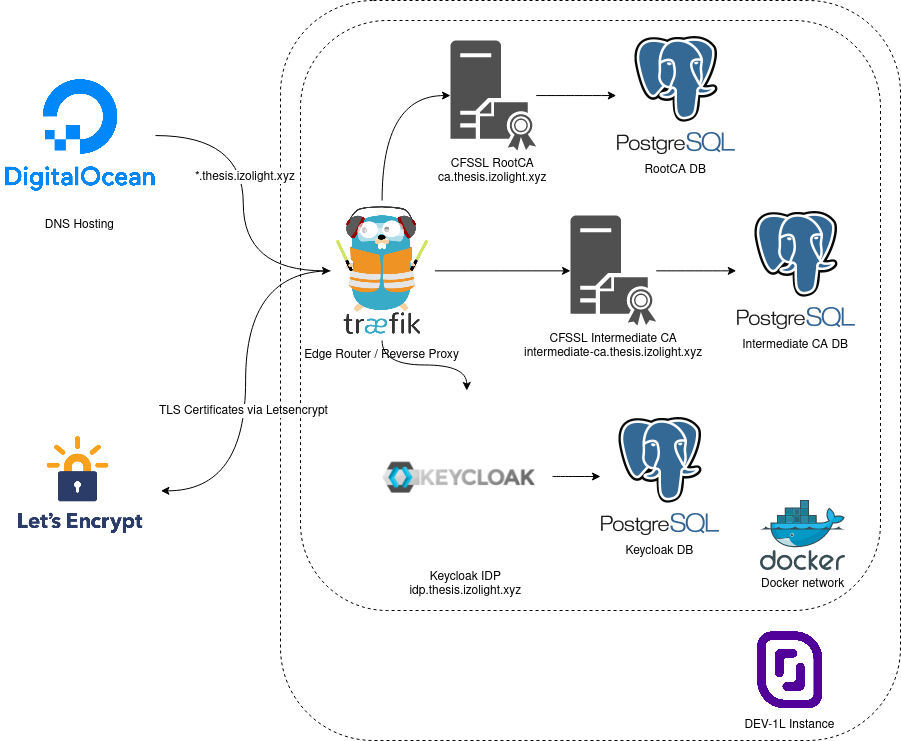
\includegraphics[width=0.9\linewidth]{images/infrastructure.png}
    \caption{Infrastructure Big Picture}
    \label{fig:infrastructurebigpicture}
\end{figure}

\begin{figure}
    \begin{center}
        \begin{tabular}{p{3.4cm}|p{5.7cm}|p{6.2cm}}
            \textbf{Name} & \textbf{Command} & \textbf{Ports} \\
            \hline
            traefik & /entrypoint.sh --docker\ldots & 0.0.0.0:80->80/tcp, 0.0.0.0:443->443/tcp \\*
            \hline
            keycloak & /opt/jboss/tools/docker-entrypoint\ldots & 127.0.0.1:8080->8080/tcp, 8443/tcp \\*
            \hline
            keycloak-db & docker-entrypoint.sh postgres & 5432/tcp \\*
            \hline
            cfssl-root & cfssl serve -db-config=/data/cfssl/\ldots & 8888/tcp \\*
            \hline
            cfssl-root-db & docker-entrypoint.sh postgres & 127.0.0.1:5432->5432/tcp \\*
            \hline
            cfssl-intermediate & cfssl serve -db-config=\ldots & 8888/tcp \\*
            \hline
            cfssl-intermediate-db & docker-entrypoint.sh postgres & 127.0.0.1:5433->5432/tcp \\*
            \hline
            cfssl-root-ocsp & cfssl ocspserve -address=0.0.0.0\ldots & 8888/tcp \\*
            \hline
            cfssl-intermediate-ocsp & cfssl ocspserve -address=\ldots & 8888/tcp \\*
        \end{tabular}
        \captionof{table}{Docker containers running on our POC server\label{tbl:docker}}
    \end{center}
\end{figure}

\section{Method of Work}\label{sec:method-of-work}
Two people hacking away at a shared project each on their own rarely works out well.
If we're lucky the code produced might even work, but it's probably going to be of low quality,
and there's risk of duplication of effort,
coordination and communication difficulties,
as well as exceeding deadlines.

This is why before starting work, we agreed upon a minimum of methodology.

\subsection{Version Control for Source Code}\label{subsec:version-control-for-source-code}
We put all source code under version control, in a shared repository.
This way each student can see what the other person is working on,
and the thesis advisors can keep an eye on what we're doing.
The commit log comes in handy for documenting the work timeline after the fact as well,
and it's a way of backing up our work.
Thankfully \gls{BFH} offers its students a Gitlab instance~\cite{gitlab}, so we will be using that.

\subsection{Standardised Build Tools and Environment}\label{subsec:standardised-build-tools-and-environment}
Few things are more annoying in a developer's life than troubleshooting build failures.
One developer adds a dependency, installs it on their machine, and forgets to tell the others.
Another developer updates their system and now uses a later version of a library, causing incompatibilities.

Furthermore,
our advisors most likely aren't very keen on installing the toolchains necessary for building our artefacts on their own machines,
they'd rather directly examine the results.

This is why a standardised, centralised build environment is a good thing to have.
Since \gls{BFH} is so kind as to offer us Gitlab runners toghether with their Gitlab instance~\cite{gitlab},
we will use that.
We've set up build pipelines based on Docker images to build our components as well as the documentation each time new commits are pushed to the master branch.
Figure~\ref{fig:gitlabcijobs} contains a screenshot of what this looks like in Gitlab's web interface.

\begin{figure}
    \begin{center}
        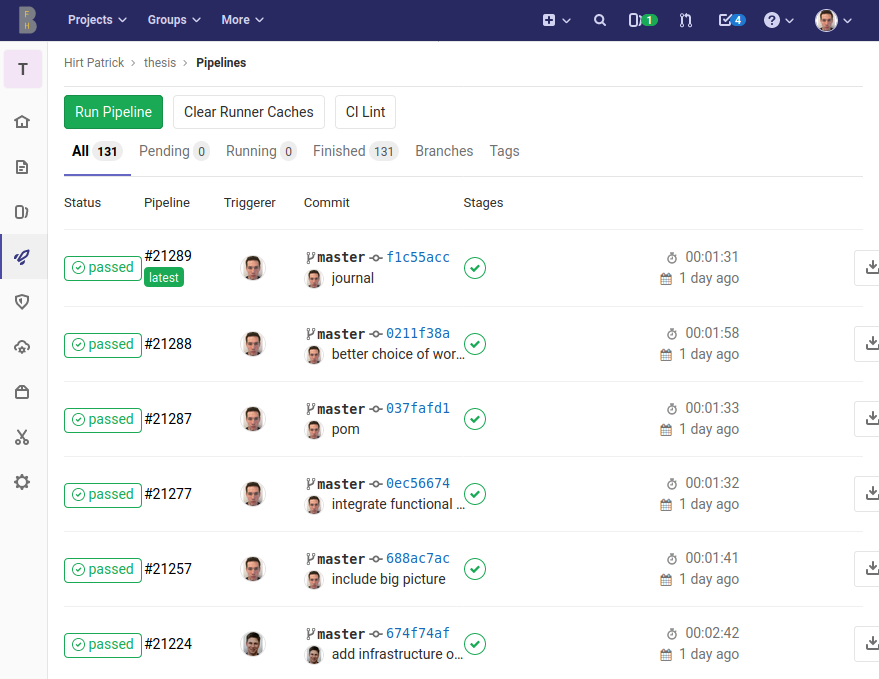
\includegraphics[width=0.8\linewidth]{images/gitlabcijobs.png}
        \caption{Gitlab CI Jobs}
        \label{fig:gitlabcijobs}
    \end{center}
\end{figure}

\subsection{Subdividing Work Packages}\label{subsec:subdividing-work-packages}
To be able to plan and schedule our work efficiently,
we divided the work packages into user stories,
as is customary in SCRUM.
We again used Gitlab for filing, planning and tracking the user stories.
Gitlab's issue system isn't exactly meant for use with SCRUM,
but we've managed to adapt it by using it as follows:
\begin{itemize}
    \item Issues are used for User Stories
    \item Labels are used for tracking progress ("todo", "doing", "done")
    \item Milestones are used for Sprint boundaries
\end{itemize}
Together with the issue board view used as a Storyboard view,
this works quite well for smaller projects such as ours.
Figure~\ref{fig:scrumboard} contains a screenshot of what this looks like.

\begin{figure}
    \begin{center}
        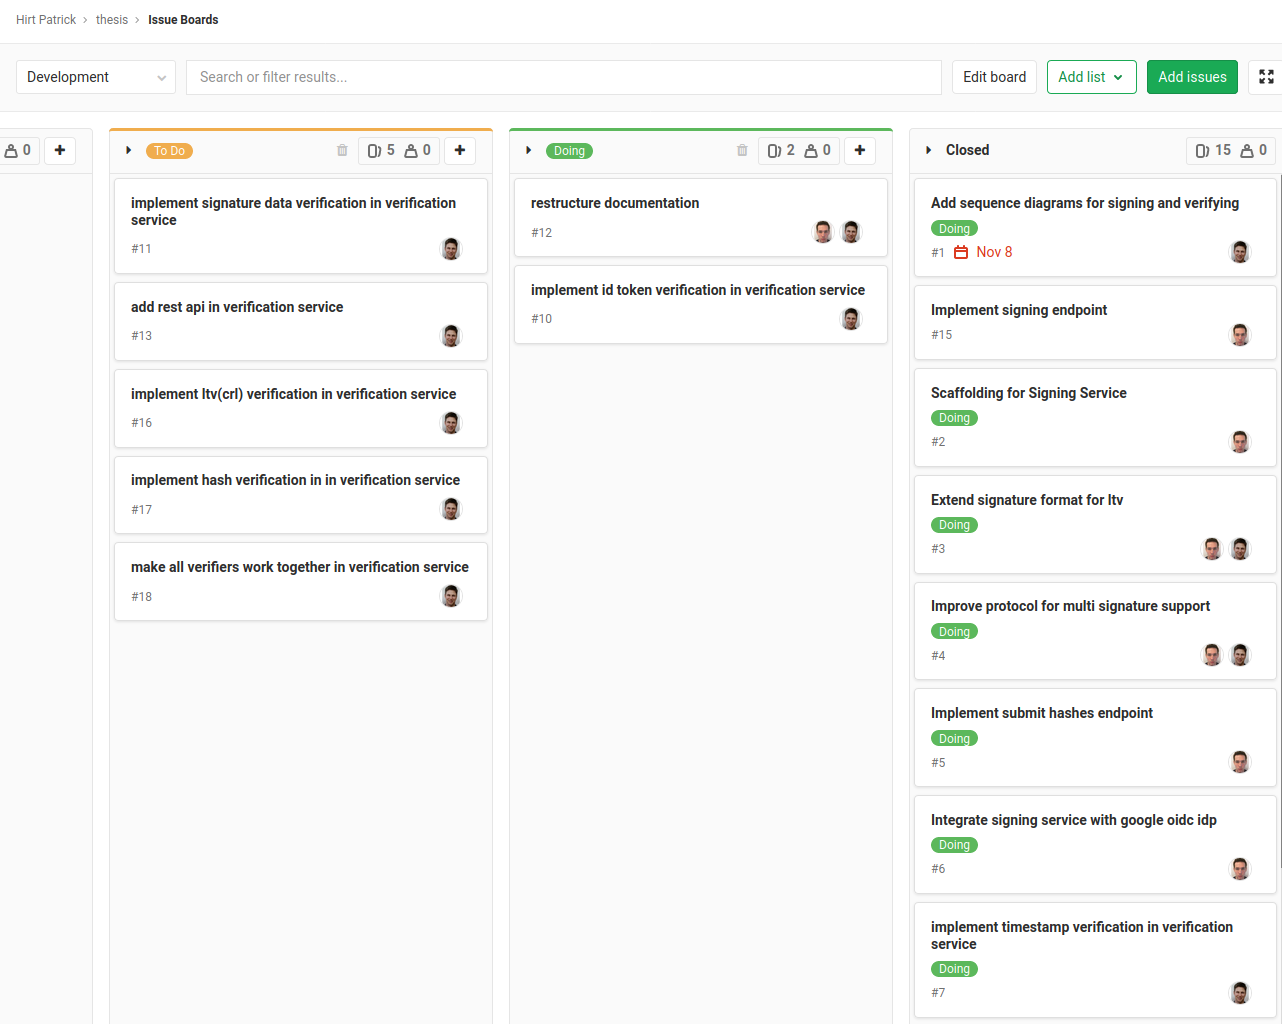
\includegraphics[width=0.8\linewidth]{images/board.png}
        \caption{SCRUM Storyboard}
        \label{fig:scrumboard}
    \end{center}
\end{figure}

\subsection{Tracking Progress}\label{subsec:tracking-progress}
In addition to the commit log and the Storyboard,
we kept an informal work log in the repository so that our advisors can check up on our progress effortlessly
any time they want.
On top of that we met with them regularly during the whole work,
discussing the progress, potential issues and of course to receive regular feedback.

\subsection{Test Coverage}\label{subsec:test-coverage}
For the signing server, we achieve a test coverage of 86.4\%,
as measured by the Intellij coverage runner.
This value, while respectable, isn't that as high as we'd like.
We inspected the coverage report and found that this is mainly due to deserialisation code in data classes that must take fields that are never used.
Excluding these classes, we achieve a coverage of 94.9\%.
TODO coverage of verifier.


